%%%%%%%%%%%%%%%%%%%%%%%%%%
% MSc Project Background Report Template
% Prof. Roger K. Moore
% University of Sheffield
% 22 March 2017
%%%%%%%%%%%%%%%%%%%%%%%%%%


\documentclass[11pt,oneside]{book}
\usepackage[margin=1.2in]{geometry}
\usepackage{setspace}
\usepackage[toc,page]{appendix}
\usepackage[none]{hyphenat} % turn hyphenation off by default
\usepackage{graphicx}
\usepackage{float}

\begin{document}

\frontmatter

\begin{titlepage}

% You need to edit the details here
\begin{center}
{\LARGE University of Sheffield}\\[1.5cm]
\linespread{1.2}\huge {\bfseries A tool to specify testable causal models of software behaviour}\\[1.5cm]
\linespread{1}

\includegraphics[width=5cm]{images/tuoslogo.png}\\[1cm]
{\Large Hao-Hsuan Teng}\\[1cm]
{\large \emph{Supervisor:} Dr Neil Walkinshaw}\\[1cm]
{\Large COM3610}\\[1cm]
\large A report submitted in fulfilment of the requirements\\ for the degree of BSc in Software engineering\\[0.3cm] 
\textit{in the}\\[0.3cm]
Department of Computer Science\\[2cm]
\today
\end{center}

\end{titlepage}

% -------------------------------------------------------------------
% Declaration
% -------------------------------------------------------------------

\newpage
\chapter*{\Large Declaration}

\setstretch{1.1} % set the line spacing differently if you wish, but this looks good to me. 

All sentences or passages quoted in this report from other people's work have been specifically acknowledged by clear cross-referencing to author, work and page(s). Any illustrations that are not the work of the author of this report have been used with the explicit permission of the originator and are specifically acknowledged. I understand that failure to do this amounts to plagiarism and will be considered grounds for failure in this project and the degree examination as a whole.\\[1cm]

\noindent Name : Hao-Hsuan Teng\\[1mm]
\rule[1em]{25em}{0.5pt}

\noindent Signature : Hao-Hsuan Teng\\[1mm]
\rule[1em]{25em}{0.5pt}

\noindent Date : 11/5/2022\\[1mm]
\rule[1em]{25em}{0.5pt}

% -------------------------------------------------------------------
% Abstract
% -------------------------------------------------------------------

\chapter*{\Large \center Abstract}

Lorem ipsum dolor sit amet, consectetuer adipiscing elit. Aenean commodo ligula eget dolor. Aenean massa. Cum sociis natoque penatibus et magnis dis parturient montes, nascetur ridiculus mus. Donec quam felis, ultricies nec, pellentesque eu, pretium quis, sem. Nulla consequat massa quis enim. Donec pede justo, fringilla vel, aliquet nec, vulputate eget, arcu. In enim justo, rhoncus ut, imperdiet a, venenatis vitae, justo. Nullam dictum felis eu pede mollis pretium. Integer tincidunt. Cras dapibus. Vivamus elementum semper nisi. Aenean vulputate eleifend tellus. Aenean leo ligula, porttitor eu, consequat vitae, eleifend ac, enim. Aliquam lorem ante, dapibus in, viverra quis, feugiat a, tellus. Phasellus viverra nulla ut metus varius laoreet. Quisque rutrum. Aenean imperdiet. Etiam ultricies nisi vel augue. Curabitur ullamcorper ultricies nisi. Nam eget dui. Etiam rhoncus. Maecenas tempus, tellus eget condimentum rhoncus, sem quam semper libero, sit amet adipiscing sem neque sed ipsum. Nam quam nunc, blandit vel, luctus pulvinar, hendrerit id, lorem. Maecenas nec odio et ante tincidunt tempus. Donec vitae sapien ut libero venenatis faucibus. Nullam quis ante. Etiam sit amet orci eget eros faucibus tincidunt. Duis leo. Sed fringilla mauris sit amet nibh. Donec sodales sagittis magna. Sed consequat, leo eget bibendum sodales, augue velit cursus nunc.


% -------------------------------------------------------------------
% TOC etc
% -------------------------------------------------------------------

\tableofcontents
\listoffigures 
\setstretch{1.1} 

\mainmatter

\chapter{Introduction}
Throughout the years, companies have developed CPU with more and more powerful processing power, and these more powerful CPU comes the invention of supercomputer, these supercomputers have superior computational power compared to normal computers. With this computational power, people start to develop large and complex computational models. Computational model is a way to try and use computer system to simulate real life situation, these models use large amounts of parameters to determine the behavior or outcomes of a certain event, researchers can utilize these models to simulate experiments and real-life event \cite{Reference1} and aid their research with the results.\\*\\*
But these models aren’t without problems, one problem is these models has large number of inputs and outputs, and it takes a lot of times to process the. This means in order to test them, it also requires a lot of time to test all inputs and outputs’ accuracy with traditional method \cite{Reference2}. \\*\\*
There are several advanced testing techniques or tools that have been developed, but these techniques or tools usually require specific knowledge in software testing. Causcumber is one of those tools and is the tool this project mainly built upon. Causcumber is a tool that can determines the relationship between different input and output parameters and use this information to create graphs that focus on certain behaviours. Then just simply compare the difference between the test sets and the output of the tested models, people can know how accurate a certain interaction is between input and output parameters. With this method tester can saved a lot of time compared to traditional method where the best ways to test it is to run the model repeatedly with new data \cite{Reference3}. \\*\\*
The problem with this method is that there’s currently lack of a user-friendly way for people to access Causcumber, it requires a level of knowledge in software testing to understand how to operate this tool. The solution provided by this project is to implement a tool as a medium, this tool minimizes the need for user to interact with the programming part of the testing process. Instead of require user to interact with the code directly, it visualizes the code into a way that is easy to read for user, highlight the parts that require edit and prompt what to edit for user. With this tool, testing with Causcumber become more accessible for people who don’t have extensive knowledge in software testing. \\*\\

\section{Aims and Objectives}
This project will be primary based on Causcumber, a tool for testing computational model and is mainly based on a model called Covasim, Covasim is a computational model focus on COVID-19 analyses, it can determine the infection rate and how will the rate change based on different interventions (such as quarantine, social distance, etc.) \cite{Reference4}. Causcumber is a in developing tool and is aimed to provide a testing method for computational model like Covasim, it uses Cucumber specification, another tool reads executable specification in plain text and validates if the software does what those specifications say, to produce casual model graph. \\*\\*
Since Causcumber is a new system that is still in development, there isn’t a convenient way for user to interact with the system. So, the primary goal of this project is to provide a tool that can streamline the testing process, minimize the need to interact with programming code directly, allowed users to get a grasp of how to use this system more easily. \\*\\*
Another goal of this system is that it needs to be easy to read, and to achieve this, we use gherkin reference to help with it, by using a set of special keywords with a certain structure, it can give meaning to executable specifications. For the users who are not specialize in software engineering, this is a way to make the system easy to understand and can avoid a lot of confusion. \\*\\*

\section{Overview of the Report}

In the next chapter, Literature Survey, a list of literature will be providing information and reasons why there’s a need for this type of testing tool to exist. It will start with explaining what scientific software is, and what are their purpose. Follow up with why they are hard to test and why they aren’t usually tested in a proper method. Then provide some of the current testing methods and why those methods are insufficient. Then this will be followed up with introductions to Cucumber and Behave, two of the main factors of the Causcumber system. After that will be explain what Causal testing is and how computational model testing is could benefit from it. Finally, explaining the current flaw of this method and what can be done to improve it.\\* \\* 
In the third chapter, Requirements and Analysis, will be mainly talking about the requirements and objectives of the system. And what solution is possible based on these requirements\\* \\*
Part four, Design, will be discussing the design philosophy of the system, the design process and discuss what the system should do. \\* \\*
Part five, Implementation and testing, will be demonstrate the final system by introduce different parts of it and what functions do those parts have. \\* \\*
Part six, Evaluation, will provide two walkthrough of testing process with different models using the implemented user interface, each walkthrough will include the full testing process, the results, and a discuss about the result.\\* \\*
Part seven, Conclusions, will summarize what has been achieved in this project, provide a overview on how the final product performs.







\chapter{Literature Survey}

Lorem ipsum dolor sit amet, consectetuer adipiscing elit. Aenean commodo ligula eget dolor. Aenean massa. Cum sociis natoque penatibus et magnis dis parturient montes, nascetur ridiculus mus. Donec quam felis, ultricies nec, pellentesque eu, pretium quis, sem. Nulla consequat massa quis enim. Donec pede justo, fringilla vel, aliquet nec, vulputate eget, arcu. In enim justo, rhoncus ut, imperdiet a, venenatis vitae, justo. Nullam dictum felis eu pede mollis pretium. Integer tincidunt. Cras dapibus. Vivamus elementum semper nisi. Aenean vulputate eleifend tellus. Aenean leo ligula, porttitor eu, consequat vitae, eleifend ac, enim. \cite{Reference2} Aliquam lorem ante, dapibus in, viverra quis, feugiat a, tellus. Phasellus viverra nulla ut metus varius laoreet. Quisque rutrum. 
\begin{equation}
M = \frac{1}{T}\sum_{t=1}^{T} e(t) / \max_{t}[e(t)]
\end{equation}
Aenean imperdiet. Etiam ultricies nisi vel augue. Curabitur ullamcorper ultricies nisi. Nam eget dui. Etiam rhoncus. Maecenas tempus, tellus eget condimentum rhoncus, sem quam semper libero, sit amet adipiscing sem neque sed ipsum. Nam quam nunc, blandit vel, luctus pulvinar, hendrerit id, lorem. Maecenas nec odio et ante tincidunt tempus. Donec vitae sapien ut libero venenatis faucibus. Nullam quis ante. Etiam sit amet orci eget eros faucibus tincidunt. Duis leo. Sed fringilla mauris sit amet nibh. Donec sodales sagittis magna. Sed consequat, leo eget bibendum sodales, augue velit cursus nunc.

\section{A Section that Contains a Figure}

Lorem ipsum dolor sit amet, consectetuer adipiscing elit. Aenean commodo ligula eget dolor. Aenean massa. Cum sociis natoque penatibus et magnis dis parturient montes, nascetur ridiculus mus. Donec quam felis, ultricies nec, pellentesque eu, pretium quis, sem. Nulla consequat massa quis enim \cite{Reference1}. Donec pede justo, fringilla vel, aliquet nec, vulputate eget, arcu. In enim justo, rhoncus ut, imperdiet a, venenatis vitae, justo. Nullam dictum felis eu pede mollis pretium. Integer tincidunt. Cras dapibus. 
\begin{figure}[ht]
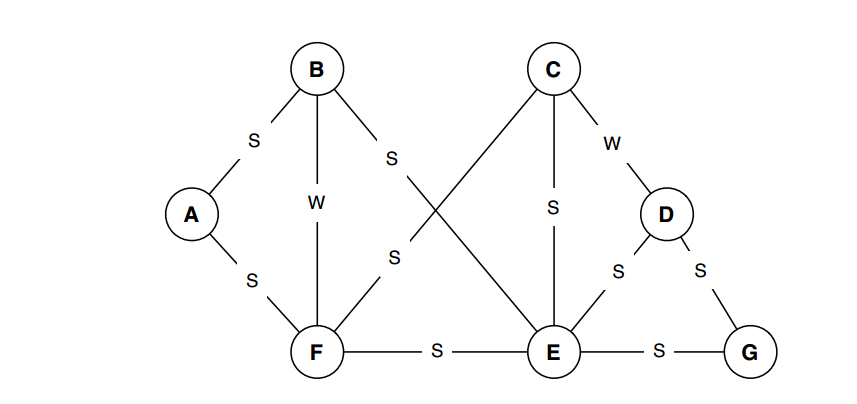
\includegraphics[width=15cm]{figures/figure1.png}
\caption{A simple figure in \LaTeX. Reproduced from http://tinyurl.com/nqtrlj5 with the permission of the copyright owner.}
\label{fig:graph}
\end{figure}
Porttitor eu, consequat vitae, eleifend ac, enim. Aliquam lorem ante, dapibus in, viverra quis, feugiat a, tellus. Phasellus viverra nulla ut metus varius laoreet. Quisque rutrum. Aenean imperdiet. Etiam ultricies nisi vel augue. Curabitur ullamcorper ultricies nisi. Nam eget dui. Etiam rhoncus. Maecenas tempus, tellus eget condimentum rhoncus, sem quam semper libero, sit amet adipiscing sem neque sed ipsum. Nam quam nunc, blandit vel, luctus pulvinar, hendrerit id, lorem. See Figure \ref{fig:graph}. Maecenas nec odio et ante tincidunt tempus. Donec vitae sapien ut libero venenatis faucibus. Nullam quis ante. Etiam sit amet orci eget eros faucibus tincidunt. Duis leo. Sed fringilla mauris sit amet nibh. Donec sodales sagittis magna. Sed consequat, leo eget bibendum sodales, augue velit cursus nunc.

\section{A Section that Contains a Table}

Lorem ipsum dolor sit amet, consectetuer adipiscing elit. Aenean commodo ligula eget dolor. Aenean massa. Cum sociis natoque penatibus et magnis dis parturient montes, nascetur ridiculus mus. Donec quam felis, ultricies nec, pellentesque eu, \cite{Reference3} pretium quis, sem. Nulla consequat massa quis enim. Donec pede justo, fringilla vel, aliquet nec, vulputate eget, arcu. In enim justo, rhoncus ut, imperdiet a, venenatis vitae, justo. Nullam dictum felis eu pede mollis pretium. Integer tincidunt. Cras dapibus. Vivamus elementum semper nisi. Aenean vulputate eleifend tellus. Aenean leo ligula, 

\begin{table}[ht]
\center
\begin{tabular}{cc|c}
A & B & A XOR B\\
\hline
0 & 0 & 0\\
0 & 1 & 1\\
1 & 0 & 1\\
1 & 1 & 0\\
\end{tabular}
\caption{A simple table in \LaTeX.}
\label{tab:xor}
\end{table}

porttitor eu, consequat vitae, eleifend ac, enim. Aliquam lorem ante, dapibus in, viverra quis, feugiat a, tellus. Phasellus viverra nulla ut metus varius laoreet. Quisque rutrum. Aenean imperdiet. Etiam ultricies nisi vel augue. Curabitur ullamcorper ultricies nisi. Nam eget dui. Etiam rhoncus. Maecenas tempus, tellus eget condimentum rhoncus, sem quam semper libero, sit amet adipiscing sem neque sed ipsum. See Table \ref{tab:xor}. Nam quam nunc, blandit vel, luctus pulvinar, hendrerit id, lorem. Maecenas nec odio et ante tincidunt tempus. Donec vitae sapien ut libero venenatis faucibus. Nullam quis ante. Etiam sit amet orci eget eros faucibus tincidunt. Duis leo. Sed fringilla mauris sit amet nibh. Donec sodales sagittis magna. Sed consequat, leo eget bibendum sodales, augue velit cursus nunc.

\section{Summary}

Lorem ipsum dolor sit amet, consectetuer adipiscing elit. Aenean commodo ligula eget dolor. Aenean massa. Cum sociis natoque penatibus et magnis dis parturient montes, nascetur ridiculus mus. Donec quam felis, ultricies nec, pellentesque eu, pretium quis, sem. Nulla consequat massa quis enim. Donec pede justo, fringilla vel, aliquet nec, vulputate eget, arcu. In enim justo, rhoncus ut, imperdiet a, venenatis vitae, justo. Nullam dictum felis eu pede mollis pretium. Integer tincidunt. Cras dapibus. Vivamus elementum semper nisi. Aenean vulputate eleifend tellus. Aenean leo ligula, porttitor eu, consequat vitae, eleifend ac, enim. Aliquam lorem ante, dapibus in, viverra quis, feugiat a, tellus. Phasellus viverra nulla ut metus varius laoreet. Quisque rutrum. Aenean imperdiet. Etiam ultricies nisi vel augue. Curabitur ullamcorper ultricies nisi. Nam eget dui. Etiam rhoncus. Maecenas tempus, tellus eget condimentum rhoncus, sem quam semper libero, sit amet adipiscing sem neque sed ipsum. Nam quam nunc, blandit vel, luctus pulvinar, hendrerit id, lorem. Maecenas nec odio et ante tincidunt tempus. Donec vitae sapien ut libero venenatis faucibus. Nullam quis ante. Etiam sit amet orci eget eros faucibus tincidunt. Duis leo. Sed fringilla mauris sit amet nibh. Donec sodales sagittis magna. Sed consequat, leo eget bibendum sodales, augue velit cursus nunc.

\chapter{Analysis}
Computational models are often to large and complex for traditional method to test, this cause developers of those models unwilling to test their models thorough. Furthermore, computational model developer are often scientist or researchers that don’t have extent knowledge in software engineering or software testing. Due to the different training receive by scientist compared to software developer, the importance of software testing is often overlooked.  \\*
Causal model testing can be a powerful tool to test computational model, but for people don’t have specific knowledge in software engineering, causal model testing can be hard tool to use. Causal model testing requires software testers to integrate the causal model with software model that is being tested, consider the complexity of the computational model being tested can be, it is hard to integrate the test into it for non-software engineer tester. There’s currently a lack of user-friendly way to test computational model with causal model testing, it is possible to integrate behave and cucumber to make this easier for people, by integrate Cucumber tester can use easy to understand language to specify the testing process and behave can read and execute these processes. By combining all these researchers who want to test their computational model can have an easy to access tool to test their software.
\begin{center}
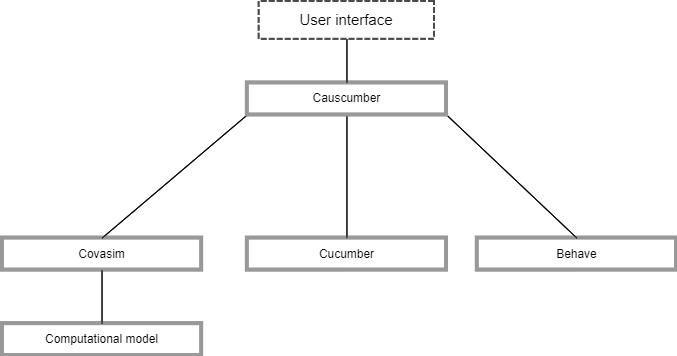
\includegraphics[width=12cm]{figures/Analysis.png}\\
Figure 2. A diagram analysis for the system
\end{center}
\section{Project Requirements}

The main goal of this project is to develop an easy-to-use system where people can use it the execute the feature file they have written, the system will exam the feature file and go through the computational model to check if the model perform as the test specify. As a result, the system should produce a coherent result detailing the accuracy of the tested model. Thus, the systems need to accomplish the following:\\*
1.	As a user, I want this system to be easy to understand, when I use the system, I want to immediate know what I need to do to get the result I want.\\*
2.	As a user, I want the system to go through the feature file I provide and test the computational model with it.\\*
3.	As a user, I want the system to produce a result where I can know the accuracy of the computational model.\\*
Since there’s already a tool been in developing for a while called Causcumber, a modify version of cucumber for testing computational model, what this project aims to accomplish is adding more to this tool. Currently the state of Causcumber is capable of execute some feature files that use to test a computational model named Covasim. And it is capable of returning lot of useful information, but the information still requires some organization to make the result easier to read. And currently there isn’t a way to execute the testing system without using the terminal to execute the command, so there’s a need of a user interface for people to operate the system. Last is that currently the only way to create a feature file is by hand type the files, and this might cause some error or confusion. Therefore, by the end of the project Causcumber should be able to accomplish the following:\\*
1.	As a user, I want the result produce by the system to be clean and easy to understand, focusing on the important part.\\*
2.	As a user, I want to execute and interact with the system through a user interface.\\*
3.	As a user, I want to have a more convenient way to create a feature file, to avoid any mistake during the creation of the feature file.\\*


\section{Ethical, Professional and Legal Issues}

Lorem ipsum dolor sit amet, consectetuer adipiscing elit. Aenean commodo ligula eget dolor. Aenean massa. Cum sociis natoque penatibus et magnis dis parturient montes, nascetur ridiculus mus. Donec quam felis, ultricies nec, pellentesque eu, pretium quis, sem. Nulla consequat massa quis enim. Donec pede justo, fringilla vel, aliquet nec, vulputate eget, arcu. In enim justo, rhoncus ut, imperdiet a, venenatis vitae, justo. Nullam dictum felis eu pede mollis pretium. Integer tincidunt. Cras dapibus. Vivamus elementum semper nisi. Aenean vulputate eleifend tellus. Aenean leo ligula, porttitor eu, consequat vitae, eleifend ac, enim. Aliquam lorem ante, dapibus in, viverra quis, feugiat a, tellus. Phasellus viverra nulla ut metus varius laoreet. Quisque rutrum. Aenean imperdiet. Etiam ultricies nisi vel augue. Curabitur ullamcorper ultricies nisi. Nam eget dui. Etiam rhoncus. Maecenas tempus, tellus eget condimentum rhoncus, sem quam semper libero, sit amet adipiscing sem neque sed ipsum. Nam quam nunc, blandit vel, luctus pulvinar, hendrerit id, lorem. Maecenas nec odio et ante tincidunt tempus. Donec vitae sapien ut libero venenatis faucibus. Nullam quis ante. Etiam sit amet orci eget eros faucibus tincidunt. Duis leo. Sed fringilla mauris sit amet nibh. Donec sodales sagittis magna. Sed consequat, leo eget bibendum sodales, augue velit cursus nunc.

\chapter{Design}
In order to satisfy the requirement, the design of the user interface will focus on making it easy to navigate and understand. It will also need to have the ability to help user create new testing scenario.
\section{Design background}
Since the basic version of Causcumber require user to manually coded in every step, this tool will be focus on reengineer it into a more accessible version. In Causcumber, user will need to define various file to test a model, first user will need to create a scenario folder, this folder should contain all the file required for user to test a model, then user will need to define four files. First is a \textsl{.dot} file, this file will define the relations of parameter for files. Second is the \textsl{environment.py}, in this file user will need to define a function that allows user to execute the tested computational mode. Next is \textsl{dag\_steps.py} and \textsl{abstract.py}, user will need to define multiple methods so that when user execute a feature file, Causcumber can execute the correct test. After all these is done, user can then define feature file, in the feature file, user will first need to define the background, then the edges for the model, last is the scenario outline and scenario where user define parameter change and expected outcome.\\*\\*
This tool should modify the information provide by the tester into the files and format above so Causcumber can read. This system is under the assumption that its users have knowledge in programming, but isn’t specialize in this area, especially not trained in software testing \cite{Reference11}. Another problem this tool needs to tackle is the lack of will to test a model due to how tedious it is, so testing step will need to be concise and straight to the point. To achieve this, the design of the system should focus on making testing part of the system as streamlined as possible, and the result is produced concise and easy to read.

\section{Design concept and process}
Since the tool need to satisfy the requirements, the design of the interface will need to accomplish the following:\\*
\\*
1.	The ability to create new scenario\\*
\\*
2.	The ability to select existing scenario\\*
\\*
3.	The ability to auto generate essential files for a scenario\\*
\\*
4.	The ability to create Dot file for scenario\\*
\\*
5.	The ability to create Feature file for the scenario\\*
\\*
In order to make this system easy to use, all the function should be straight forward, and there should be guide provided for the user to refer to. \\*\\*
In the main screen, it should allow user to select which feature file they wish test and run the test and produce the result. This screen should also provide a portal to other function provided by this interface such creating dot and feature file, below is a design concept for this part:

\begin{figure}[H]
	\centering
	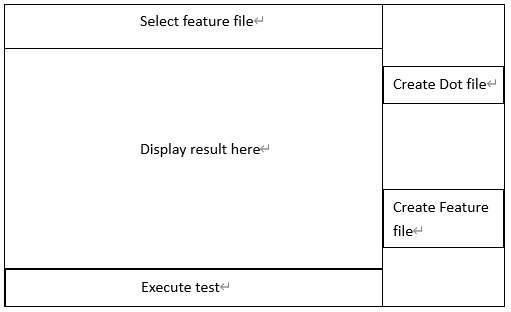
\includegraphics[width=10cm]{figures/mainMenu.png}\\
	\caption{Design concept for main menu.}
	\label{fig:figure4}
\end{figure}
\noindent 
To test model, first user will need to create a .dot file that define the relation of the parameters. By select the create .dot file option in the menu, the user will be bought to a screen that can edit what parameters is in the model. To make this function even more convenient, there should be a way to visualize the relation of the parameters. By visualize the relation of the parameter, user can use it as a reference to aid them in the process. User will also need to edit the relation between them, next screen will need to display the parameters the user previous entered. The user can select what a parameter is related to, and like the previous part, the interface will also have a visualization to assist user, below is a design concept for this part:

\begin{figure}[H]
	\centering
	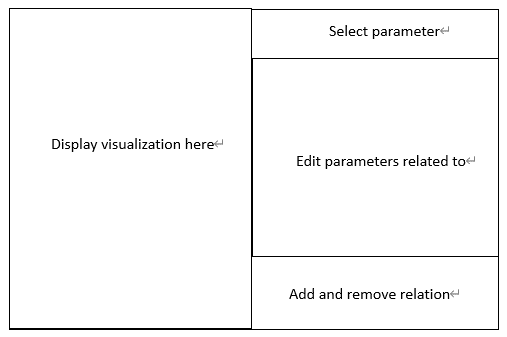
\includegraphics[width=10cm]{figures/editDot2.png}\\
	\caption{Part 2.Design concept for edit .dot function.}
	\label{fig:figure6}
\end{figure}
\noindent 
After edit the relation of parameter, user will need to edit the auto generated files, \textsl{environment.py}, \textsl{dag\_steps.py} and \textsl{abstract.py}, to run the model and read the output, the purpose of these file is for Causcumber to execute the tested model and read the information provided by the model. This part assumed the user have certain level of knowledge in programming, that they have to ability to modify those files\\*\\*
When all the setup process is done, user can start creating feature file as test case, user can select the edit feature file function from the main screen edit it. This function will be structured in a way that is easy to navigate and mostly represent how the final feature file will look like. Since feature file are more complex compared to .dot file, there are more steps required to accomplished this process. \\*\\*
First, user need to define the parameters, parameter type and its value, this setup the tested parameter and their value. User will also need to define what parameter needs to be record. Below is a design concept for this part: 

\begin{figure}[H]
	\centering
	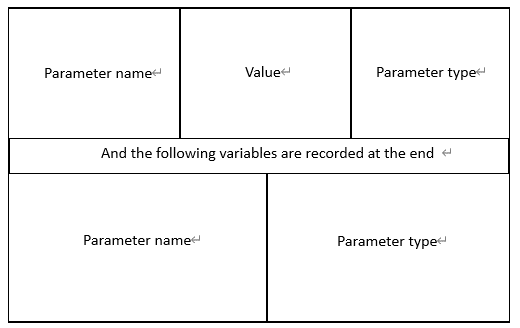
\includegraphics[width=10cm]{figures/editFeature1.png}\\
	\caption{Part 1.Design concept for edit .feature function.}
	\label{fig:figure7}
\end{figure}
\noindent 
Then, user will need to define edges for the parameters entered in the first part, this part should be similar to the previous edit .dot part to keep the consistence of the system, with some minor change.\\*\\*
Finally, user can start defining the scenarios. In scenarios, user can define a certain situation such as increase the value of a certain variable, and what the expect outcome of the system will be, visualization is also provide to assist user in the process. Below is a design concept for this part:

\begin{figure}[H]
	\centering
	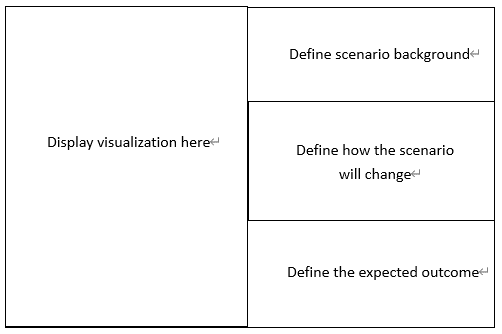
\includegraphics[width=10cm]{figures/editFeature2.png}\\
	\caption{Part 2.Design concept for edit .feature function.}
	\label{fig:figure8}
\end{figure}






\chapter{Implementation and testing}
Following the design, the implementation aimed to fulfill it and the requirements. Some changes were made to the implementation according to the feed back of the Causcumber team. Since Causcumber are built with python, this tool will also be built will python to reduce the chance of any potential problem happening. The tool will primary be a front end for Causcumber, and it will be built with Kivy, an open source python library mainly for develop user interface and application \cite{Reference20}. 

\section{Overview}
This project will utilize the Screen and ScreenManager function in Kivy. This design is due to many steps in testing with Causcumber require different syntax, to make this clearer for user, different syntax is assigned to different screen. With this, different screen will have different composition to reflect each syntax, extra functions are added to some screens to assist user in editing. This design also allows the development process be more efficient and concise. Since if there’s any new function required to be added, develop can simply create a new screen with new function and use ScreenManager to connect it to existing screen, and the new function can be organized into file(s) to keep the codes concise. Since Causcumber require several mandatory files to work, user will need to go through several steps before execute the test, below is the basic workflow of the tool:
\begin{figure}[H]
	\centering
	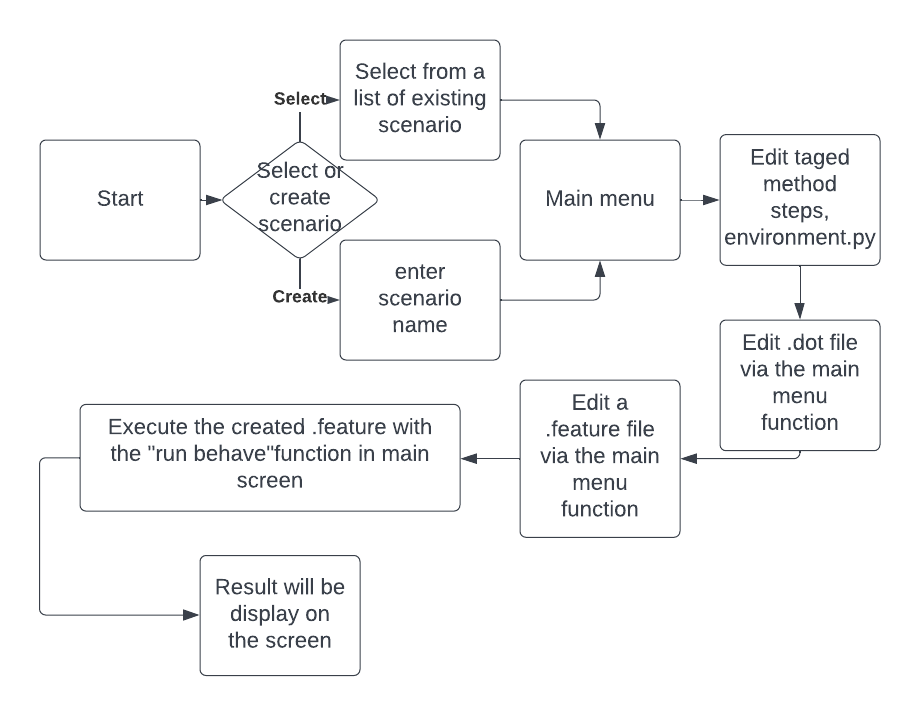
\includegraphics[width=10cm]{figures/workFlow.png}\\
	\caption{Basic workflow for testing a model.}
	\label{fig:figure9}
\end{figure}


\section{Create and select scenario}
In the beginning, Causcumber require user to create scenario directory, a scenario contains two mandatory sub-directories, \textsl{dags}, a directory contain causal graphs that defines the relations of parameter as \textsl{.dot} file. The second sub-directories is \textsl{features}, a directory where user can create \textsl{.feature} file that contain element for behave \cite{Reference21}. It also contain \textsl{environment.py} file, and a sub-directory \textsl{steps} that has scripts to implement step definitions for \textsl{.feature} file. The tool will allow user to create or select and existing scenario, upon create a new scenario, the tool will generate the basic files and sub-directory required for a scenario. Upon starting the system, the user will have two options, select, and create scenario.
\begin{figure}[H]
	\centering
	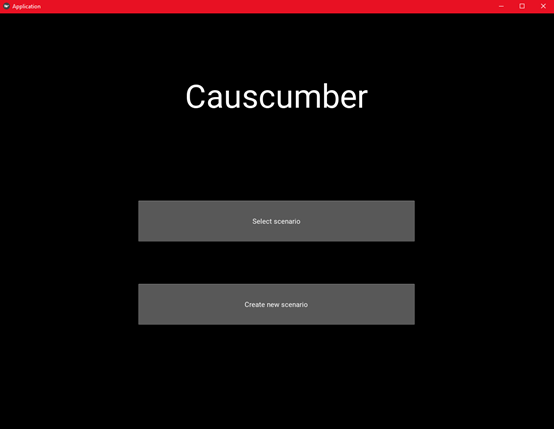
\includegraphics[width=10cm]{figures/startScreen.png}\\
	\caption{Start screen.}
	\label{fig:figure10}
\end{figure}
If user choose to select existing scenario, they will be presented with a list of existing scenarios to choose from. If user choose to create a new scenario, user will be prompt to enter the scenario name.
\begin{figure}[H]
	\centering
	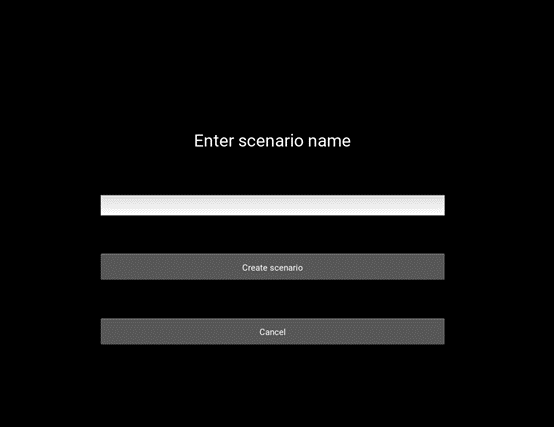
\includegraphics[width=10cm]{figures/createNewScenario.png}\\
	\caption{Create new scenario screen.}
	\label{fig:figure11}
\end{figure}
The tool will create files with custom file and method name based on the scenario name entered by the user.

\section{Main screen}
In the basic version of Causcumber, to execute test, user will need to use terminal and run the command “behave feature/{feature filename}”. In the main screen, user can achieve this by simple use the “Select feature file” to chose the target \textsl{.feature} file, and “run behave” to execute the test. Then the result will be display on the screen. But before this, user will need to go through some steps to setup the test.
\begin{figure}[H]
	\centering
	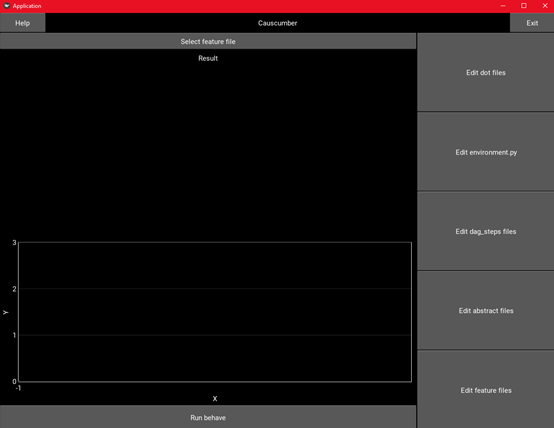
\includegraphics[width=10cm]{figures/mainScreen.png}\\
	\caption{Main screen.}
	\label{fig:figure12}
\end{figure}
The steps required is placed from top to bottom at the right of the screen as shown above, user will need to finish all the steps in order to test a model. A help section on top left is also provided to guide user if needed.

\section{Edit .dot file}
In the \textsl{.dot} file, user will first need to define the parameter clusters, typically there will be two clusters, one for input parameters and another for output parameters. After that user will need to define the relation between the parameters, this is done by using the syntax \textsl{ parameter1 -> parameter2}. One useful feature for \textsl{.dot} file is combine with Graphviz, an open source graph visualization software, user can generate a graph that help visualize the relation and cluster. 
\begin{figure}[H]
	\centering
	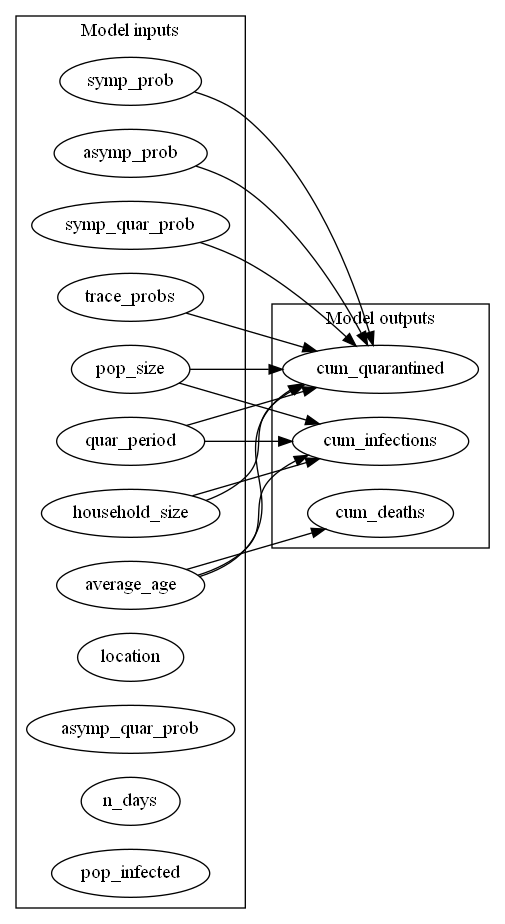
\includegraphics[width=10cm]{figures/dotExample.png}\\
	\caption{Graphviz example.}
	\label{fig:figure13}
\end{figure}
In the user interface, Graphviz is used to assist in the process. After click on the “Edit dot files” button in the menu, user will be brought to the screen for editing parameter clusters. 
\begin{figure}[H]
	\centering
	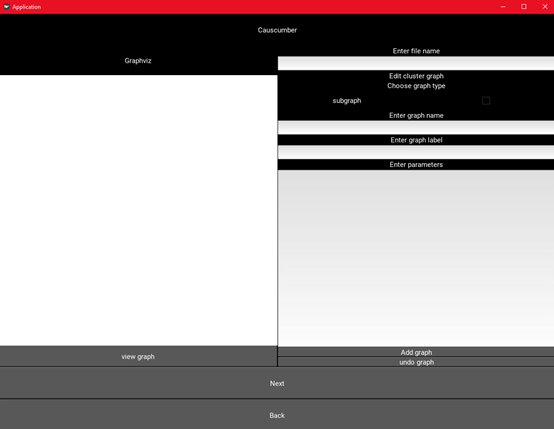
\includegraphics[width=10cm]{figures/editDot1Screen.png}\\
	\caption{Add parameter to .dot file.}
	\label{fig:figure14}
\end{figure}
At the right side, user will need to enter the filename, this can either be an existing file or a new file. Next user can change the syntax of the graph by tick or untick the subgraph checkbox, after user will need to enter the graph name and label. Then in the last section, enter parameters, user can enter the parameter for the graph.\\*\\*
After user input all the parameters, user can click next to go to the next step to edit relation of the parameters. Same as before, user should enter the filename, after that user need to click on the “Update parameter relation”, then the interface will display parameters entered in the previous step. By clicking the “select parameter”, a drop down menu will open for user to select a parameter, by select a parameter, that mean the selected parameter is related to the parameters ticked below (Include itself if ticked). When finish editing relations, user can click the “add graph” button to input the graph. The result of the graph will be display at the left side of the screen to assist the user. 
\begin{figure}[H]
	\centering
	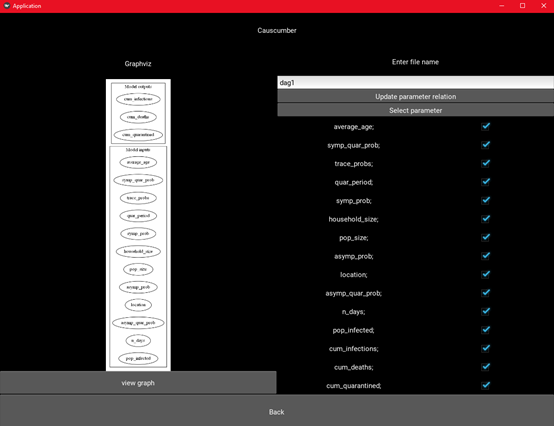
\includegraphics[width=10cm]{figures/editDot2Screen.png}\\
	\caption{Edit parameter relation.}
	\label{fig:figure15}
\end{figure}

\section{Setup background files}
Next, there are three background files require to setup. First in \textsl{environment.py}, user need to edit a \textsl{run\_[Model name]} method, the purpose of this file is to execute the testing model, user will need to modify it to able to run the model and return the result data. Second, is in \textsl{dag\_steps.py}, there are two parts require to be edit, custom distributions and metavariables. \\*\\*
For custom distributions, user is requiring to define class for distributions so that Causcumber can picks it up. The reason for why this needed is because default distributions in Causcumber uses SciPy, an open-source software for mathematics, science, and engineering \cite{Reference22}, to generate valid parameters values between 0 and 1, but not all the parameters are numerical. Custom distributions are for these types of parameters, for example \textsl{location} in covasim, custom distributions should generate strings from a given set.\\*\\*
For metavariables, user can define metavariables in the Background. Metavariables, or metasyntactic variable in computer science is a placeholder name that has no meaning and will be substituted \cite{Reference23}. User can use this to modify data in data sets.\\*\\*
The third file is \textsl{abstract.py}, in this file user can define custom constrains for parameter value. This limits the distributions for test data generation. For all three files, it requires users to manually define it since different models may work differently and require different codes, use uniform generated codes may cause problem. In the main screen, buttons are provided to help user open these file, by clicking those button, the files will be open with default editor set by the user.

\section{Edit .feature files}
Finally, user can start edit the feature file. In feature file, user will need to define background, list edges, scenario outline and scenario. In background, user will need to define the parameters and the distribution, user can also define metavariables, then user will need to define variables are recorded at the end, last user can also define extra conditions for the scenario with \textsl{And} syntax in Cucumber. \\*\\*
In the next part, user will need the list the edges of models, this part allow Causcumber to focus on relations of parameters in model define by the user. Next is \textsl{Scenario outline}, in this part user can define changes in parameter and the expected outcome, this require user to provide \textsl{Example}. Finally is \textsl{Scenario}, this is mostly same as \textsl{Scenario outline} but without  \textsl{Example}.\\*\\*
All the parts mentioned above require user to formatted in a certain syntax, with the interface, the syntax is incorporated into the format of the interface’s design. Starting with background, user need to edit the feature file’s name, then user can start setting the parameters, parameters’ type and parameters’ value. Next user can add meta variables, this part isn’t necessary for feature file, and can be left empty. Next is the recorded variables, this part is similar to the meta variables but will generate different syntax upon create feature file. Last is the for user to add extra condition to the background if needed. This part is structured very similar to the \textsl{.feature} file’s syntax, but with some modification to make those syntax even more plain text.
\begin{figure}[H]
	\centering
	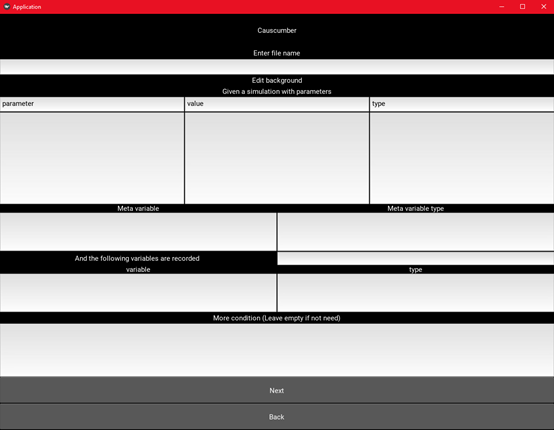
\includegraphics[width=10cm]{figures/editFeature1Screen.png}\\
	\caption{Edit first section of .feature file.}
	\label{fig:figure16}
\end{figure}
Next part is to define the edges, this part is mostly identical to the edit \textsl{.dot} function to keep the consistence of the system, the only new addition is a new option allow user to add new edges. This new function is added due to the potential need for user to add extra edges, user can choose to not add new edges if there’s no need for that.\\*\\*
After this is scenario outline and scenario, both are also structured like background, where parts of the sentence that require user to edit being left blank. In scenario outline, the syntax for example is a table like structure, this is simulated in the interface where user can use the add column and add row to edit the example. 
\begin{figure}[H]
	\centering
	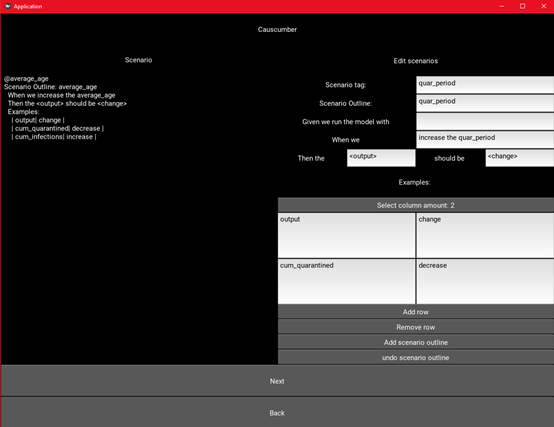
\includegraphics[width=10cm]{figures/editFeature2Screen.png}\\
	\caption{Edit scenario outline section of .feature file.}
	\label{fig:figure17}
\end{figure}
In scenario, instead of example, it uses “Then” and “And” structure in Cucumber to represent the expected result. The structure is similar to the previous page but with example replaced with the option to add “And”.
\begin{figure}[H]
	\centering
	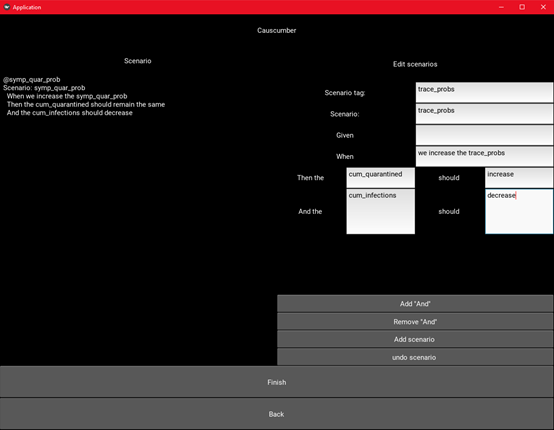
\includegraphics[width=10cm]{figures/editFeature3Screen.png}\\
	\caption{Edit scenario section of .feature file.}
	\label{fig:figure18}
\end{figure}
When done, user can just click “Finish” button to return to main menu, then select and run the feature file created.








\chapter{Evaluation}
In this chapter, the tool will be put in to test with two computational model, influenza1918 and Covasim. Influenza1918 is a relatively simple model compare to Covasim, this chapter will go through the testing process more both model, and the result produced, then some discussion about the result.
\section{Testing influenza1918}
Influenza1918 is an equation-based model originally developed to for the need to design model validation strategies, this is a model that simulate epidemiological disease-spread of the course of the 1918 Influenza epidemic within the United States.
This model has five state variables and six parameters \cite{Reference24}.
\subsection{Testing process for influenza1918}
First, a scenario name influenza1918 is created, by creating this scenario, the basic files for testing is also auto generated. Since influenza1918 is implemented through OpenModelica in a \textsl{influenza1918.mo} file, so to test this model, first user need to put the model file into the \textsl{\textbackslash scenarios\textbackslash influenza1918 \textbackslash model}. Next use the “Edit dot files” button to start edit the relations of the parameters. A file named influenza1918\_abstract is created, there are two graph needed, first is \textsl{cluster\_inputs} with the input parameters, then \textsl{cluster\_outputs} with the output parameters. In the right panel, enter the file name influenza1918\_abstract, then select the type of graph, input the graph name and label, and the parameters for the selected cluster, click add graph to apply the change.
\begin{figure}[H]
	\centering
	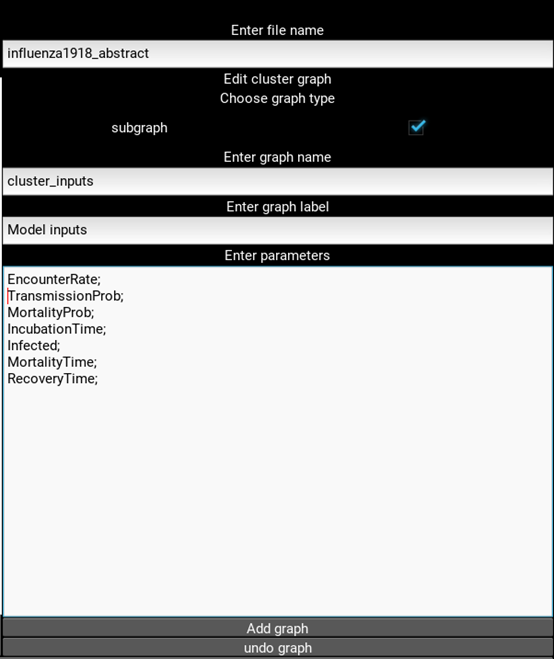
\includegraphics[width=10cm]{figures/influenzaTestProcess3.png}\\
	\caption{Edit graph for input parameters.}
	\label{fig:figure21}
\end{figure}
After added the graph, the left panel will then display the graph via Graphviz. Next is edit the relations between these parameters.
\begin{figure}[H]
	\centering
	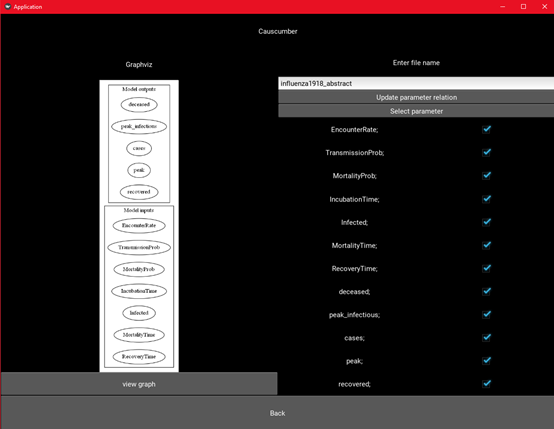
\includegraphics[width=10cm]{figures/influenzaTestProcess5.png}\\
	\caption{Edit relation for parameters.}
	\label{fig:figure23}
\end{figure}
First, select the file, then select the parameters that are going to be affected via the check-boxes, then select the parameters that are going to affect them via the drop-down menu, then the left panel will be updated.
\begin{figure}[H]
	\centering
	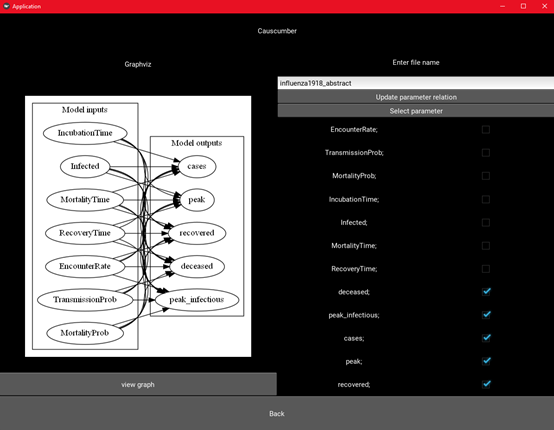
\includegraphics[width=10cm]{figures/influenzaTestProcess7.png}\\
	\caption{Relations of parameters presented in Graphviz graph.}
	\label{fig:figure25}
\end{figure}
After finishing editing the relationship, click back to return to the main menu.
Next user will need to edit the three background files. In environment.py, edit the run\_influenza1918 function to execute the influenza1918 model. Then for dag\_steps.py, define metavariables in the background, a metavariable called “m” needs a function “populate\_m” define. Last is for abstract.py file, apply custom constrain to the parameters of the tested model. \\*\\*
Finally is the \textsl{.feature} file, use “Edit feature files” to create a feature file. Starting from the top user will need to define the feature file’s name, its parameters and its value/distribution and type,
\begin{figure}[H]
	\centering
	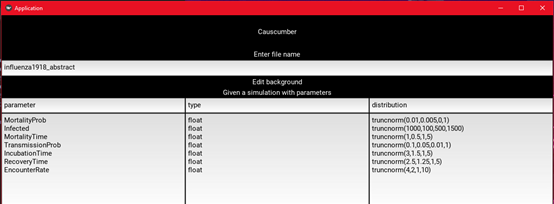
\includegraphics[width=10cm]{figures/influenzaTestProcess10.png}\\
	\caption{Edit initial parameters name, type and value/distribution in influenza1918.}
	\label{fig:figure28}
\end{figure}
Next step is to define what parameter to record and when to record, since influenza1918 doesn’t require any meta variable, that part will be left empty.
\begin{figure}[H]
	\centering
	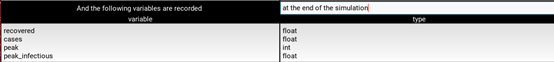
\includegraphics[width=10cm]{figures/influenzaTestProcess11.png}\\
	\caption{Edit recorded parameters name and type in influenza1918.}
	\label{fig:figure29}
\end{figure}
Next is to define the edges for the parameters, this process is same as edit dot file step. Since scenario outline is required in this case, next part will also be skip. Last is scenario, in the right panel, edit the change and expected outcome. 
\begin{figure}[H]
	\centering
	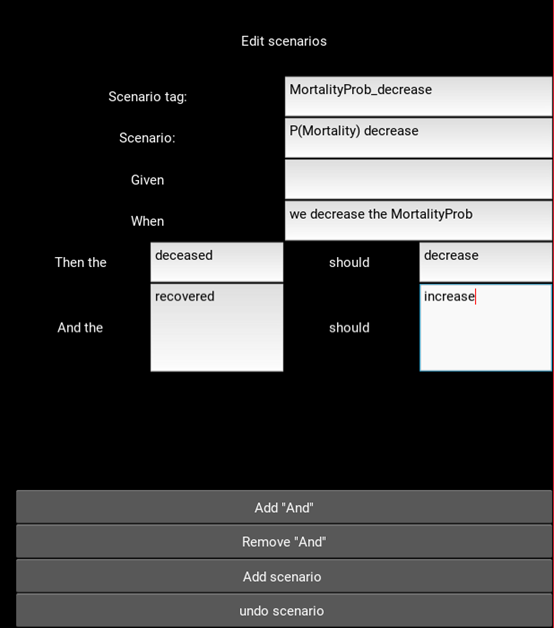
\includegraphics[width=10cm]{figures/influenzaTestProcess12.png}\\
	\caption{Edit scenario for influenza1918.}
	\label{fig:figure30}
\end{figure}
Upon finish edit all the scenario, user can then return to main menu and then select the feature file. After select feature file, user run behave to produce the result on the screen,
\begin{figure}[H]
	\centering
	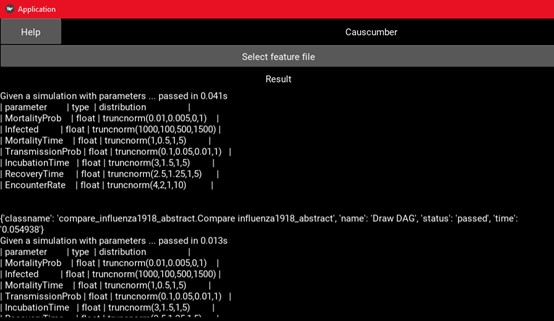
\includegraphics[width=10cm]{figures/influenzaTestProcess15.png}\\
	\caption{Result produced by Causcumber display in result section.}
	\label{fig:figure33}
\end{figure}

\subsection{Testing result for influenza1918}
In the result produced by Causcumber, either with the assisting tool or without, all produce the same result. In the files produced by the tool, starting with \textsl{.dot} file, it is identical with manually created version with some minor difference in formats that doesn’t matter in this case. With this assist of the tool, this process also become a lot more efficient. Next are the three background files, in those files, most of the parts are already pre-define with some parts that can only be manually define by user. Last, in \textsl{.feature} file, the file generated by the tool is no difference compare to the manually created file, and by splitting the files into different sections, and edit it one by one, it become more streamline and readable from a user’s point of view. 
\subsection{Discuss influenza1918 result}
With the assisting tool, creating test for influenza are relatively simplify because as a user, it is not necessary to understand all the syntax for all the files. And with the auto generated files, since not all the parts require manually input, the chance of error occur has been reduced. One of the problem originally user may encounter when define edges for files such as \textsl{.dot} file and \textsl{.feature} file, is that it is difficult for user to list all the edges without any sort of visualization. With the Graphviz’s assist, this process become much clearer during the process. Unfortunately, for the three background files, part of it still require user to manually code those parts in due to the methods use by developers to code computational model maybe drastic different.

\section{Testing Covasim}
Covasim is an agent-based model pf COVID-19 dynamics and interventions, it simulate individual people as an agent, agents will be assigned different states such as infectious or recovered, agents can change to different states and in each states can provide different affects to the simulations. Agents will also be affected by the “Interventions” such as masks or physical distancing. Compare to influenza1918 models in the previous section, this model is a lot more complex with more parameters and methods. 
\subsection{Testing process for Covasim}
First a scenario name “Covasim” is created, in this scenario, in this test, we focus on the interventions part of Covasim. Starting with \textsl{.dot} file, one graph for input parameter and another one for output is created, then the following relations are defined,
\begin{figure}[H]
	\centering
	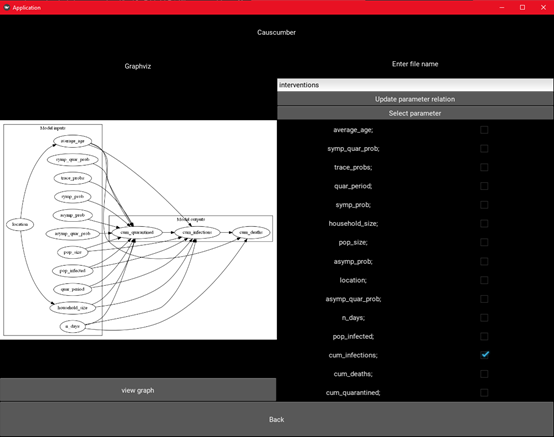
\includegraphics[width=10cm]{figures/CovasimTestProcess2.png}\\
	\caption{Relation for parameters for testing Covasim.}
	\label{fig:figure35}
\end{figure}
Next is to define the three-background file, in \textsl{abstract.py}, there are two custom constraints needs to be define, “average\_age” and “household\_size”. In covasim, one of the parameters requires string, therefore in \textsl{dag\_steps.py} a custom constrain named “countries” is defined. Next, there are several meta variables in the background, these meta variables are also defined as functions in \textsl{dag\_steps.py}. \\*\\*
Last is the feature file, in the first section, one of the parameters is location, since it only accepts string, its distribution will be using the custom distribution “countries” defined before. Also, there are meta variables require, so in this section meta variable are also required to be defined. There is also multiple extra initial condition require to be defined, this is also done in the first section.
\begin{figure}[H]
	\centering
	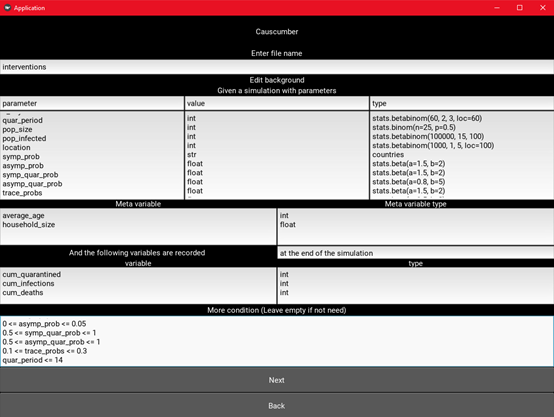
\includegraphics[width=10cm]{figures/CovasimTestProcess3.png}\\
	\caption{Background for testing Covasim.}
	\label{fig:figure36}
\end{figure}
In next section, same as influenza1918, edges are defined using the assisting tools, in Covasim, there are additional edges being added, so instead of choosing next, choose “And add edges” options to add more edges, this is similar function as define edges, but will return slightly different result in the generated feature file. Next, is to edit the scenario outline, by changing the column and row amount, we can provide information according to the requirement of the scenario outline. After this is scenarios, this process is same as influenza1918, with all these steps done, select the newly created feature file, and run Beheve.
\begin{figure}[H]
	\centering
	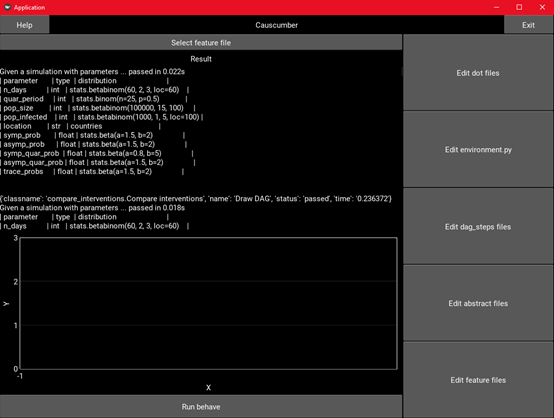
\includegraphics[width=10cm]{figures/CovasimTestProcess6.png}\\
	\caption{Result produced by using assisting tool.}
	\label{fig:figure39}
\end{figure}
\subsection{Testing result for Covasim}
In the testing result for Covasim, result produced by are similar to manually created version, in the manually created version of feature file, some Cucumber syntax can be used to reduce the length of the file, this isn’t replicate the version created by the tool. As for the test result produced by Causcumber, it is mostly identical to the manually created version with some difference in indentation which doesn’t affect the result.
\subsection{Discuss Covasim result}
In the testing process for Covasim, the tool provides a lot of assists in the process, especially in the process of defining relation of parameter, and the editing process of feature file. But with the background files, despite the guide provided, it still requires user to have decent programming skill to accomplish it. Overall, with the assist of the tool, the testing process has become more streamline and swift, but parts of the system still holds back by necessity to manually code the test.
\section{A summary of results}
In the result provided by testing on influenza1918, it shows that with the help of the tool, testing become more convenient. The process is overall simplified by reduce the need for user to directly interact with the coding part of testing. With the parts that is necessary for the process, it is mostly reduced by auto generate most of it, with some minor parts still require to be define. This is also the same when defining \textsl{.feature} file, without the need to deal with syntax and format, this process become a lot more smoother. \\*\\*
For covasim, the experience is mostly same when it comes defining relations for parameter and creating feature file, without the need to directly code these files, and with the help of the GUI, the testing process is a lot more understandable and streamline. But when it comes to the background files, despite the auto generated parts, there are still more required to be define. Consider that Covasim is a more complex model, this is to be expected, but this part also shows that if the user tends to add a lot of custom testing aspect, the testing process could still become lengthy.\\*\\*
Combine the information provide by two models, it shows that in terms of editing \textsl{.feature} file and \textsl{.dot} file. This tool can effectively assist user, but when it comes to the background file, if the user is intended to have many custom conditions, then the user will be required to do a decent amount of editing in the background files, this may discourage people to participate in testing.
\section{How does the tool help user simplify the testing process}
As shown by the result, the tool can effectively assist user by allowing user to ignore the required syntax to edit the dot and feature file, with the tool, user will only be required to input the data hinted by the GUI. In this way, user will not be required to learn the complete syntax of the file, make it easier to promote this system to people who aren’t specialize in software testing.\\*\\*
In the files that require manually input, parts of the files will be auto generated. In these files, a total of 319 lines of code will be auto generated, most of it are essential function for the working of Causcumber and will require a decent understanding in Causcumber system to implement those lines. The auto generated parts of the files, together with the assist generated dot and feature file, lowers the skill requirement to use the Causcumber.\\*\\*
To summarize, two main difficulties in using Causcumber are tackled, first is the need to understand the syntax when edit dot and feature file, second is background files for Causcumber. With these two-problem tackled, user won’t necessary need to understand how Causcumber work, but will only required to know where to input the parameters, which guides are provided to help user in the process.







\chapter{Conclusion}
Computational models are important tools in modern days, researchers and decision makers can utilize these models to aid them during research or make important decision. But these models may often receive poor testing, this is because its developers are often not trained in software testing, and the testing process can be very complex and time consuming. \\*\\*
Advance testing method are developed to assist testing, but these methods are often too complex for people who are trained in software testing. One of these tools is Causcumber, a tool that use the behaviour of model to determine if the model meet the developer’s expectation. But this tool still suffers from the same problem as other advance tool, where it maybe too complex for untrain user, therefore discourage people from using it. \\*\\*
A tool is created to improve user experience of Causcumber, this tool can automatically turn user’s input into the format that can be accepted by Causcumber, and auto generate parts of background file to reduce user’s workload. With this tool, user won’t need to learn the syntax required by Causcumber, and the line of code required user manually input is also reduced.\\*\\*
Since Causcumber is still a in development tool, and there might be changes in the future, and there’s also more to improve for the assist tool. First is in the viewing function of graphviz graph, in the current version, it’s size is limited by the some technical issues, and will affect user experience, parts of these is due some limitation of Kivy api, this will require some time to improve. \\*\\*
Second is editing scenario outline and scenario in feature file, more hints or the ability to select how the parameter going to change (For example, increase, decrease) from a menu can be implemented. This is to be decide since this function might limit the options in testing. \\*\\*
Third is to further reduce the need for user to program, namely the three background files. In those files, a similar like edit scenario in feature can be added, but since these files are a lot more complicated, the editing function for these files may not be as simple to implemented, the way user implements their model may also affect this process, which adds more complexity to the implementation of this function.\\*\\* 
Overall, this project set out to make a complex tool become more approachable, despite some technical challenges, this project provides some interesting results for more future work on this subject. With more functions implemented, testing will be more approachable in the future.



\bibliographystyle{acm} 
\bibliography{mybibliography}

\begin{appendices}
	Project Github repository : https://github.com/CITCOM-project/causcumber/tree/GUI 
\begin{figure}[H]
	\centering
	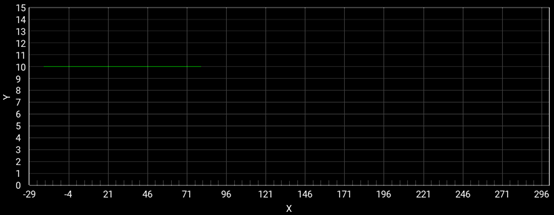
\includegraphics[width=8cm]{figures/95confidence_interval.png}\\
	\caption{A 95\% confidence interval example with one scenario passed.}
	\label{fig:figure40}
\end{figure}
\begin{figure}[H]
	\centering
	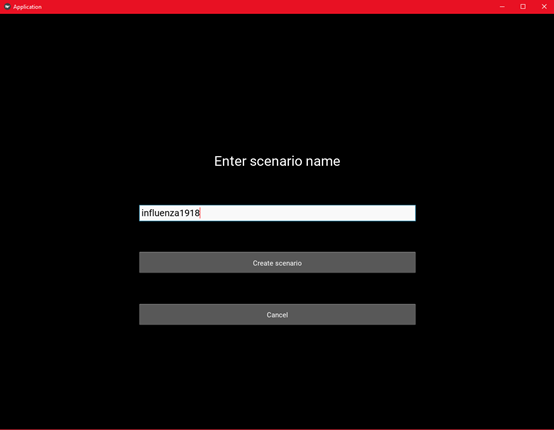
\includegraphics[width=8cm]{figures/influenzaTestProcess1.png}\\
	\caption{Creating new scenario for influenza1918.}
	\label{fig:figure19}
\end{figure}
\begin{figure}[H]
	\centering
	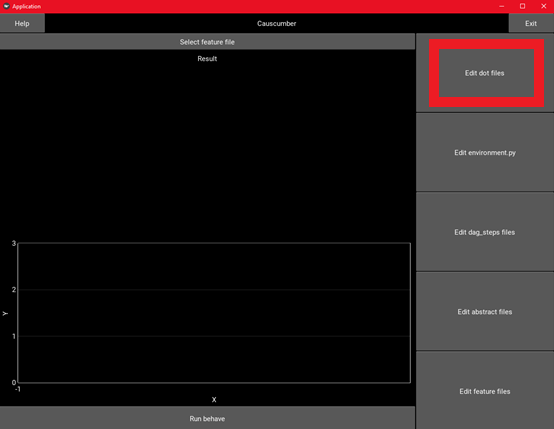
\includegraphics[width=10cm]{figures/influenzaTestProcess2.png}\\
	\caption{Select “Edit dot files” function.}
	\label{fig:figure20}
\end{figure}
\begin{figure}[H]
	\centering
	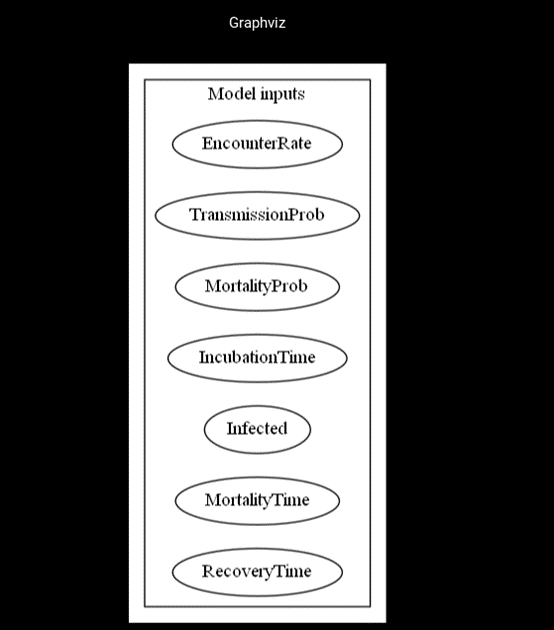
\includegraphics[width=10cm]{figures/influenzaTestProcess4.png}\\
	\caption{Graphviz for input influenza1918 parameters graph.}
	\label{fig:figure22}
\end{figure}
\begin{figure}[H]
	\centering
	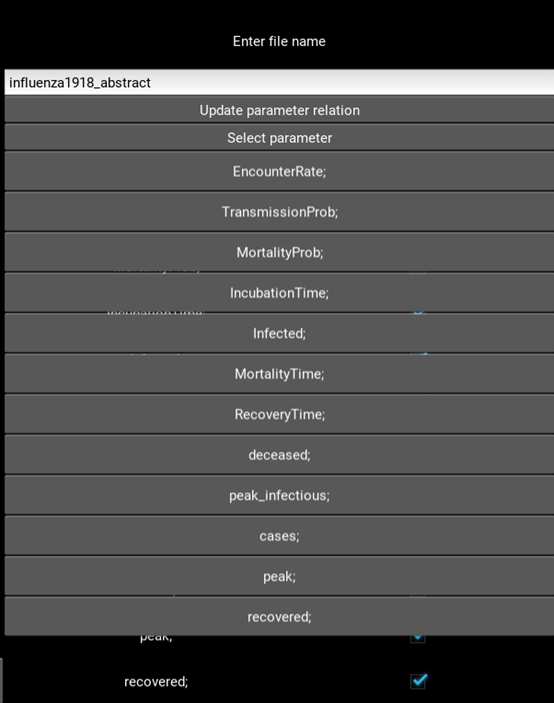
\includegraphics[width=10cm]{figures/influenzaTestProcess6.png}\\
	\caption{Drop-down menu for select parameter.}
	\label{fig:figure24}
\end{figure}
\begin{figure}[H]
	\centering
	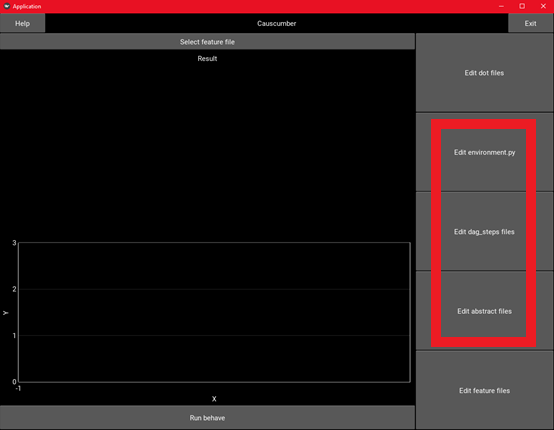
\includegraphics[width=10cm]{figures/influenzaTestProcess8.png}\\
	\caption{Edit background files for testing influenza1918.}
	\label{fig:figure26}
\end{figure}
\begin{figure}[H]
	\centering
	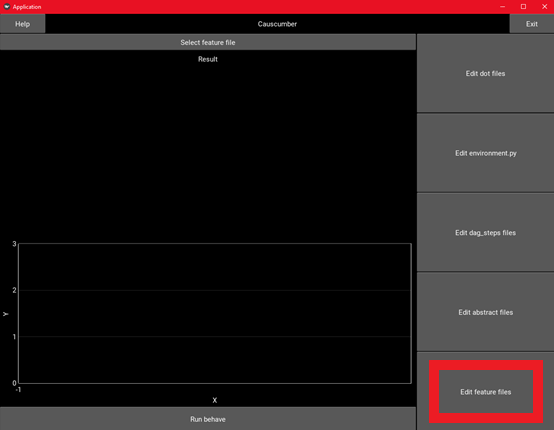
\includegraphics[width=10cm]{figures/influenzaTestProcess9.png}\\
	\caption{Edit feature files for testing influenza1918.}
	\label{fig:figure27}
\end{figure}
\begin{figure}[H]
	\centering
	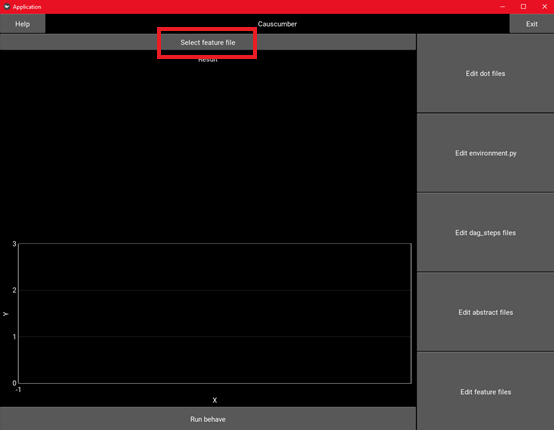
\includegraphics[width=10cm]{figures/influenzaTestProcess13.png}\\
	\caption{Select “Select feature files” function.}
	\label{fig:figure31}
\end{figure}
\begin{figure}[H]
	\centering
	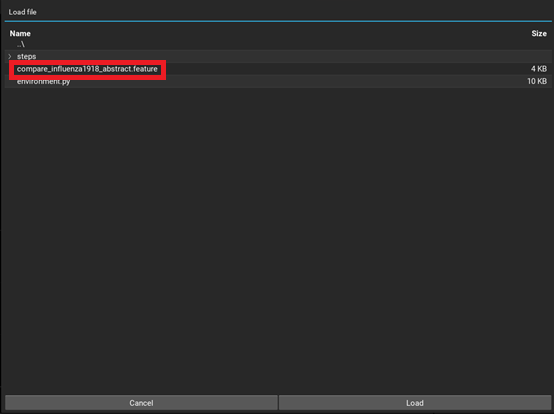
\includegraphics[width=10cm]{figures/influenzaTestProcess14.png}\\
	\caption{Select newly created feature file.}
	\label{fig:figure32}
\end{figure}
\begin{figure}[H]
	\centering
	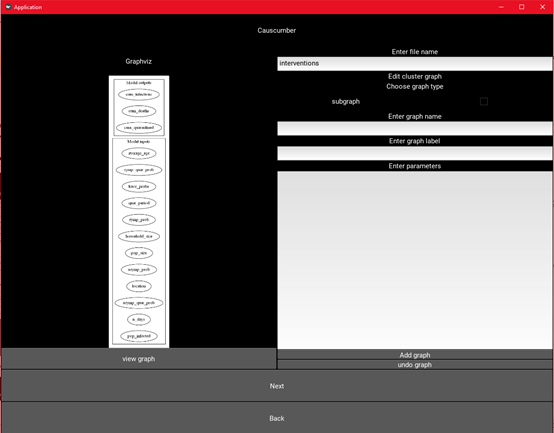
\includegraphics[width=10cm]{figures/CovasimTestProcess1.png}\\
	\caption{Input and output graph for testing Covasim.}
	\label{fig:figure34}
\end{figure}
\begin{figure}[H]
	\centering
	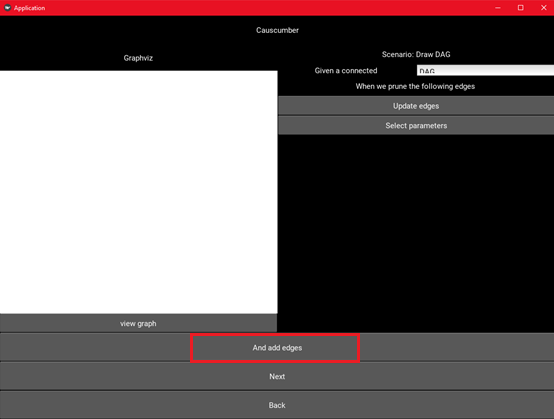
\includegraphics[width=10cm]{figures/CovasimTestProcess4.png}\\
	\caption{Select add additional edges.}
	\label{fig:figure37}
\end{figure}
\begin{figure}[H]
	\centering
	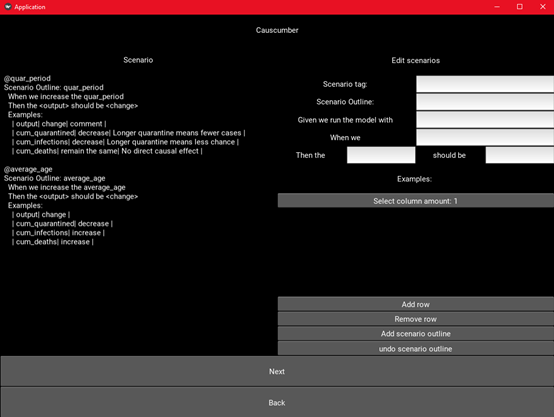
\includegraphics[width=10cm]{figures/CovasimTestProcess5.png}\\
	\caption{Scenario outline for testing Covasim.}
	\label{fig:figure38}
\end{figure}

	%\chapter{Another Appendix}

Lorem ipsum dolor sit amet, consectetuer adipiscing elit. Aenean commodo ligula eget dolor. Aenean massa. Cum sociis natoque penatibus et magnis dis parturient montes, nascetur ridiculus mus. Donec quam felis, ultricies nec, pellentesque eu, pretium quis, sem. Nulla consequat massa quis enim. Donec pede justo, fringilla vel, aliquet nec, vulputate eget, arcu. In enim justo, rhoncus ut, imperdiet a, venenatis vitae, justo. Nullam dictum felis eu pede mollis pretium. Integer tincidunt. Cras dapibus. Vivamus elementum semper nisi. Aenean vulputate eleifend tellus. Aenean leo ligula, porttitor eu, consequat vitae, eleifend ac, enim. Aliquam lorem ante, dapibus in, viverra quis, feugiat a, tellus. Phasellus viverra nulla ut metus varius laoreet. Quisque rutrum. Aenean imperdiet. Etiam ultricies nisi vel augue. Curabitur ullamcorper ultricies nisi. Nam eget dui. Etiam rhoncus. Maecenas tempus, tellus eget condimentum rhoncus, sem quam semper libero, sit amet adipiscing sem neque sed ipsum. Nam quam nunc, blandit vel, luctus pulvinar, hendrerit id, lorem. Maecenas nec odio et ante tincidunt tempus. Donec vitae sapien ut libero venenatis faucibus. Nullam quis ante. Etiam sit amet orci eget eros faucibus tincidunt. Duis leo. Sed fringilla mauris sit amet nibh. Donec sodales sagittis magna. Sed consequat, leo eget bibendum sodales, augue velit cursus nunc.

\end{appendices}
\end{document}
